% \begin{figure}[h!]
%     \centering
    
%     \begin{subfigure}{0.8\linewidth}
%         \centering
%         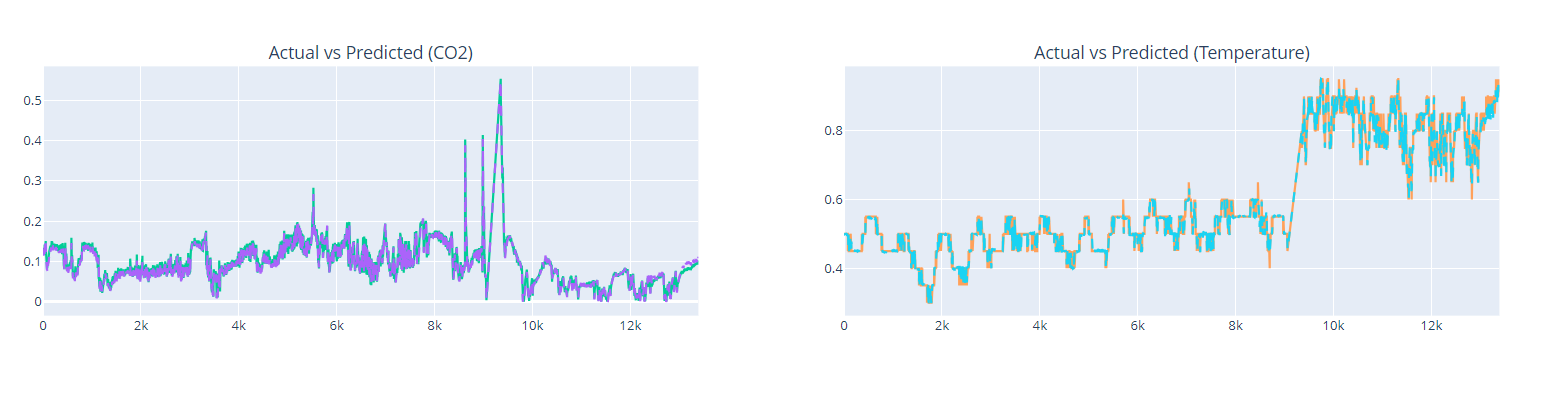
\includegraphics[width=\linewidth]{images/other actual vs predicted values.png}
%         \caption{Actual vs Predicted of \(CO_{2}\) and Temperature Over Time}
%     \end{subfigure}
    
%     \vspace{0.5cm}
    
%     \begin{subfigure}{0.8\linewidth}
%         \centering
%         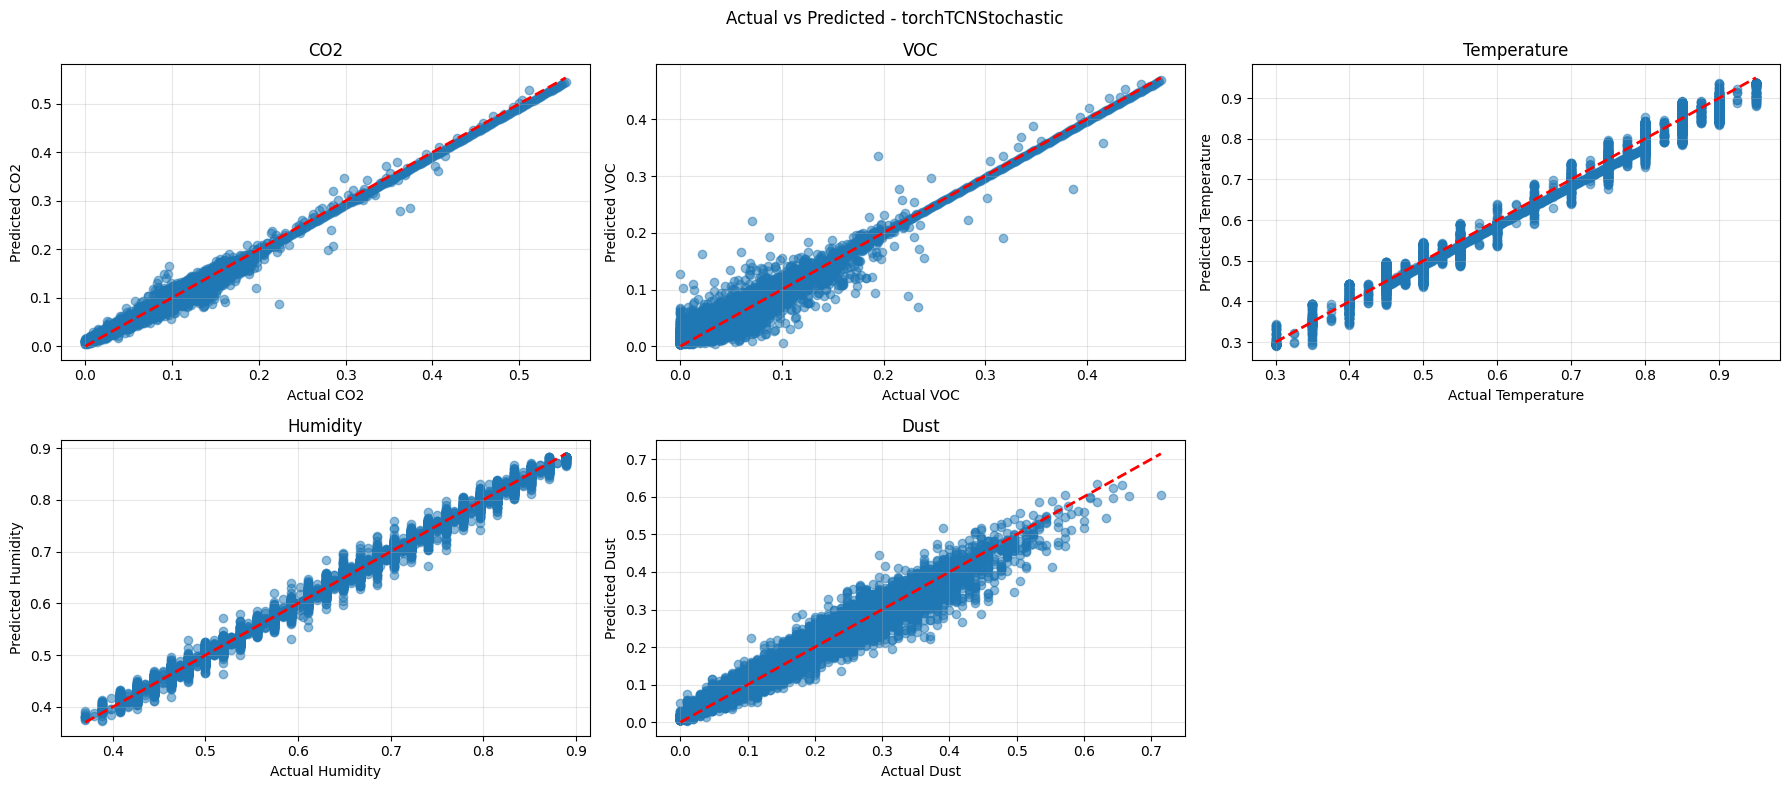
\includegraphics[width=\linewidth]{images/Actual vs predicted feature values.png}
%         \caption{Scatter Plots of Actual vs Predicted Values with Linear Regression Lines for all Parameters}
%     \end{subfigure}
    
%     \caption{Comparison of model prediction results for various variables.}
%     \label{fig:actual_vs_predicted}
% \end{figure}


\begin{figure}[h!]
    \centering
    \begin{subfigure}{0.45\linewidth}
        \centering
        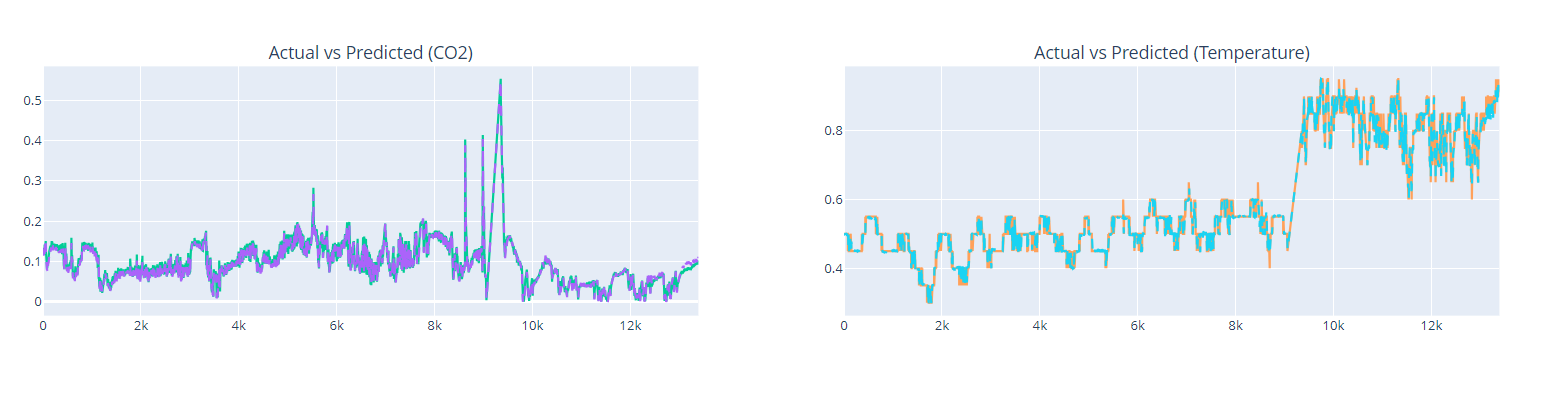
\includegraphics[width=\linewidth]{images/other actual vs predicted values.png}
        \caption{This is subfigure A}
    \end{subfigure}
    \hfill
    \begin{subfigure}{0.45\linewidth}
        \centering
        \includegraphics[width=\linewidth]{example-image-b}
        \caption{This is subfigure B}
    \end{subfigure}
    \caption{This is the main figure caption}
    \label{fig:test}
\end{figure}
